\section{\emph{Build Server}}
\label{sec:buildserver}
Dieser Abschnitt behandelt die Infrastruktur des \emph{Build}-Server Projekts in Openshift. 
Die Ressourcen für den \emph{Build Server} werden im \emph{Repository buildserver}\footnote{\url{https://github.com/OpenshiftCICD/buildserver}} verwaltet.

\subsection{\emph{Templates}}
\label{sec:openshift-templates}
Dieser Abschnitt behandelt die Openshift \emph{Templates}, welche die Services für die \emph{Build}-Server Infrastruktur definiert. Die Openshift \emph{Templates} beinhalten alle Definitionen wie z.B. \emph{BuildConfigurations} und \emph{Deployments}, die Aspekte des \emph{Core Conepts}\footnote{\url{https://docs.openshift.com/container-platform/3.5/architecture/core_concepts/index.html}} von Kubernetes und Openshift sind.\\

Diese Auflistung beschreibt die implementierten \emph{Templates}:
\begin{enumerate}
	\item Im \emph{Template} \textbf{\emph{jenkins-slaves.yml}} werden die für Jenkins zur Verfügung gestellten \emph{Slave-Container} verwaltet.
	\item Im \emph{Template} \textbf{\emph{jenkins.yml}} wird der Jenkins Service verwaltet.
	\item Im \emph{Template} \textbf{\emph{nexus.yml}} wird der Nexus3 Service verwaltet.
	\item Im \emph{Template} \textbf{\emph{pipeline.yml}} wird für das Anlegen einer Openshift \emph{Pipeline} verwendet.
\end{enumerate}

\ \subsection{Skripte}
Dieser Abschnitt behandelt die Skripten, die für das Verwalten des \emph{Clusters} verwendet werden. Mit der Applikation \emph{oc} kann mit dem \emph{Cluster} interagiert werden, wie z.B. PRojekte erstellen/löschen, oder Applikation in Projekten anlegen/löschen. Damit der \emph{Build Server} einfach erstellt oder gelöscht werden kann, sind für die Services und für den \emph{Build Server}   
Skripte erstellt worden, die alle nötigen Kommandos beinhalten.\\

Auf dem Level der Skripten wird eine Datei namens \emph{.openshift-env} erwartet, die Umgebungsvariablen definiert, die von Skripten verwendet wird.\\

Diese Auflistung beschreibt die implementierten \emph{Skripte}:
\begin{enumerate}
	\item Im \emph{Skript} \textbf{\emph{openshift-jenkins.sh}} sind alle Jenkins Service und Jenkins \emph{Slave} spezifischen Funktionen implementiert.
	\item Im \emph{Skript} \textbf{\emph{openshift-nexus.sh}} sind alle Jenkins Service und Jenkins \emph{Slave} spezifischen Funktionen implementiert.
	\item Im \emph{Skript} \textbf{\emph{openshift-buildserver.sh}} sind alle Funktionalitäten für das Verwalten des \emph{Build Servers} implementiert.
	\item Im \emph{Skript} \textbf{\emph{openshift-secrets.sh}} sind alle Funktionalitäten für das Verwalten von \emph{Secrets} implementiert. Siehe Abschnitt \ref{sec:buildserver-secrets} für eine genauere Beschreibung der verwendeten \emph{Secrets}.
\end{enumerate}

\ \subsection{Architektur}
Dieser Abschnitt behandelt den Aufbau des \emph{Build Servers}. Die Abbildung \ref{fig:architecture} zeigt, die Architektur des \emph{Build Server} Projekts in Openshift.
\begin{figure}[H]
	\centering
	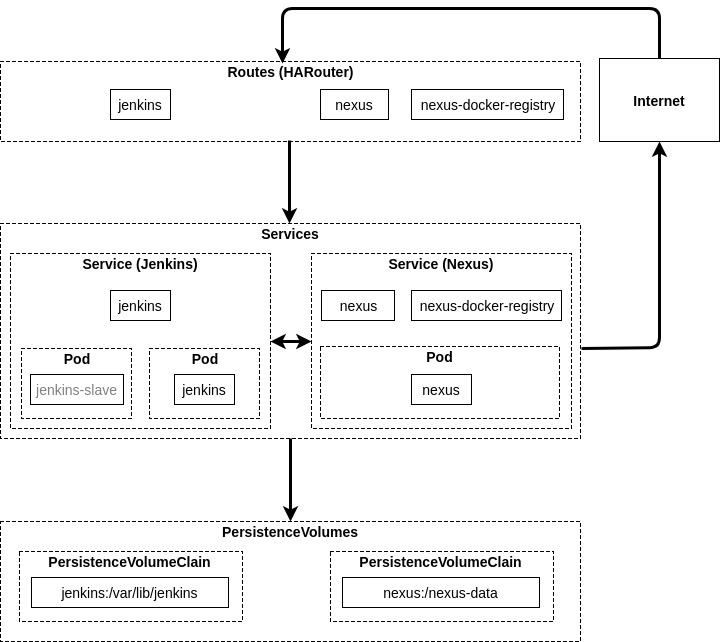
\includegraphics[scale=0.6]{logos/architecture-diagram.jpg}
	\caption{\emph{Build Server} Architektur}
	\label{fig:architecture}
\end{figure}


